\documentclass[
    11pt,
    a4paper,
    egregdoesnotlikesansseriftitles,
    toc=chapterentrywithdots,
    twoside,openright,
    titlepage,
    parskip=half,
    headings=normal,  % reduces heading size
    listof=totoc,
    bibliography=totoc,
    index=totoc,
    captions=tableheading,  % caption below table
    chapterprefix,
    listof=flat,
    final
]{scrbook}


% details about your thesis
\newcommand{\titel}{My very fancy thesis title.}
\newcommand{\artderarbeit}{Bachelorarbeit}  % {Bachelorarbeit,Masterarbeit}
\newcommand{\autor}{Georg Simon Ohm}
\newcommand{\studiengang}{Informatik}  % {Informatik,Wirtschaftsinformatik,Medieninformatik}
\newcommand{\matrikelnr}{123\,4567}
\newcommand{\erstgutachter}{Prof.\,Dr.~Korbinian Riedhammer}
\newcommand{\zweitgutachter}{Prof.\,Dr.~Bartosz von\,Rymon\,Lipinski}
\newcommand{\betreuer}{M.Sc.\,~Martina Schmidt}
\newcommand{\unternehmen}{Musterfirma GmbH}
\newcommand{\logo}{figures/TH-Nuernberg-RGB.png}
\newcommand{\keywords}{hot, fuzz}
 

% use better typography
\usepackage{microtype}

% custom head and foot
\usepackage[automark]{scrlayer-scrpage}
\pagestyle{scrheadings}
\ihead{\headmark}
\chead{}
\ohead{\pagemark}
\renewcommand*\chaptermarkformat{\chapappifchapterprefix{\ }% 
  \thechapter.\enskip}

\RedeclareSectionCommand[tocindent=0pt]{section}
\RedeclareSectionCommand[tocindent=0pt]{subsection}
%\RedeclareSectionCommand[tocnumwidth=70pt]{chapter}

\usepackage{scrhack}

% other packages
\usepackage[utf8]{inputenc}
\usepackage[T1]{fontenc}
\usepackage{lmodern,relsize,textcomp,csquotes}
\usepackage{amsmath,amsfonts}
\usepackage[ngerman,english]{babel}  % flip for German thesis
\usepackage[final]{graphicx}
\usepackage{setspace,geometry,xcolor}
\usepackage{makeidx}
\usepackage{paralist,ifthen,todonotes}
\usepackage{url}
\usepackage[toc]{glossaries}
\usepackage{pdfpages}

% table setup
\usepackage{longtable}
\usepackage{array}
\usepackage{ragged2e}
\usepackage{lscape}

% pdf hyperref
\usepackage[
    bookmarks=true,
    bookmarksopen=true,
    bookmarksnumbered=true,
    bookmarksopenlevel=1,
    pdftitle={\titel},
    pdfauthor={\autor},
    pdfcreator={\autor},
    pdfsubject={\titel},
    pdfkeywords={\keywords},
    pdfpagelabels=true,
    colorlinks=true,
    linkcolor=red,
    urlcolor=magenta,
    anchorcolor=black,
    citecolor=cyan,
    filecolor=magenta,
    menucolor=red,
    plainpages=false,
    hypertexnames=true,
    linktocpage=true,
]{hyperref}

% configure your listings style
\usepackage{listings}
\lstset{
	tabsize=3,
	extendedchars=true,
	frame=single,
	showstringspaces=true,
	numbers=left,
	numberstyle=\small,
	breakautoindent=true
}

% page setup
% \setlength{\topskip}{\ht\strutbox}
\geometry{paper=a4paper,left=2.5cm,top=3.0cm,bindingoffset=.8cm}
\onehalfspacing
\frenchspacing
\clubpenalty = 10000
\widowpenalty = 10000 
\displaywidowpenalty = 10000

% some commands
\newcommand{\ua}{\mbox{u.\,a.\ }}
\newcommand{\zB}{\mbox{z.\,B.\ }}
\newcommand{\dahe}{\mbox{d.\,h.,\ }}
\newcommand{\bzw}{\mbox{bzw.\ }}
\newcommand{\bzgl}{\mbox{bzgl.\ }}
\newcommand{\eg}{\mbox{e.\,g.\ }}
\newcommand{\ie}{\mbox{i.\,e.\ }}
\newcommand{\wrt}{\mbox{w.\,r.\,t.\ }}
\newcommand{\etal}{\mbox{\emph{et.\,al.\ }}}


% TODO remove if not needed...
\usepackage{blindtext}

% load glossary entries
\makenoidxglossaries
\loadglsentries{glossary}

\begin{document}

\setcounter{secnumdepth}{3}  % numerate subsections
\setcounter{tocdepth}{2}  % ...but don't include them in toc

\frontmatter
\include{cover}\cleardoublepage

% download the following form and complete it (hit save in your editor)
% https://intern.ohmportal.de/fileadmin/Gelenkte_Doks/Abt/SZS/SB/SB_0050_FO_Pruefungsrechtliche_Erklaerung_und_Erklaerung_zur_Veroeffentlichung_der_Abschlussarbeit_public.pdf
%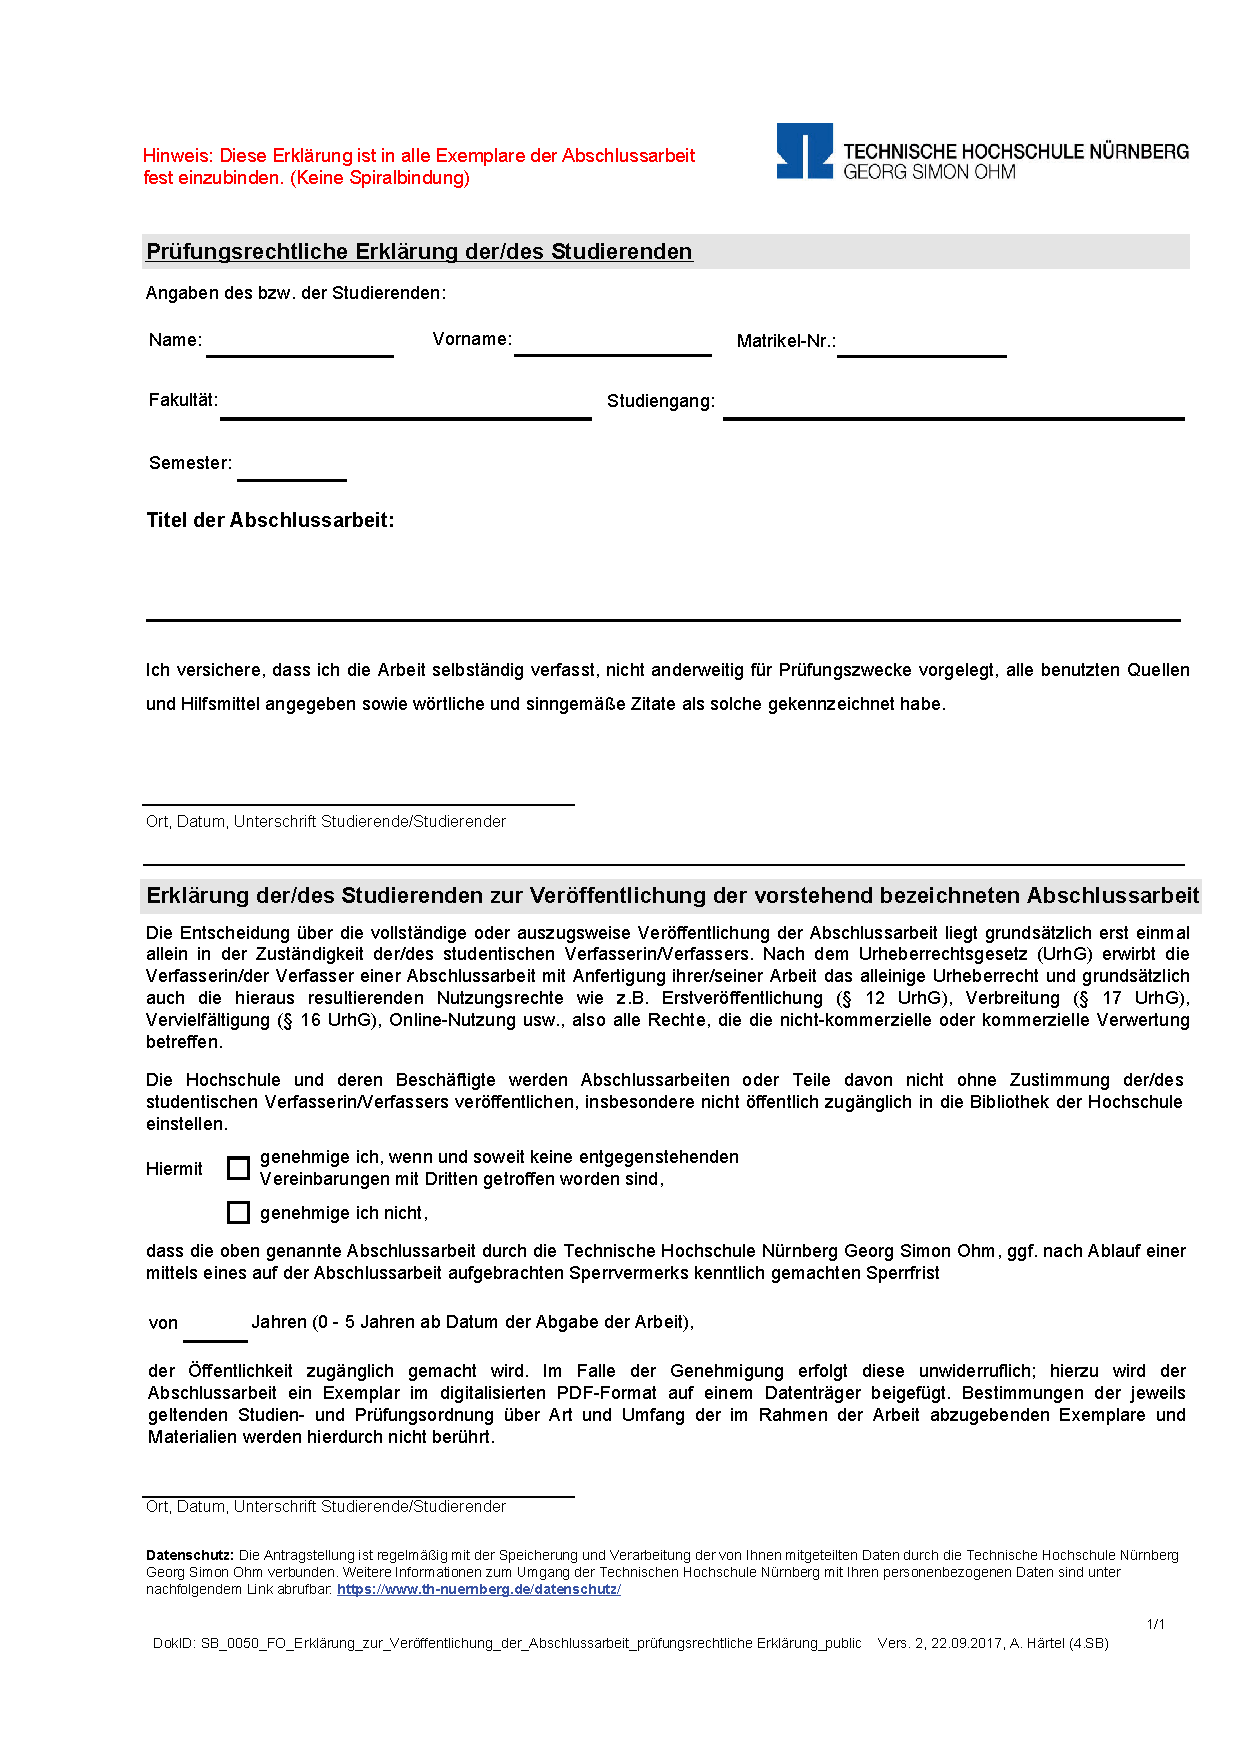
\includepdf{SB_0050_FO_Pruefungsrechtliche_Erklaerung_und_Erklaerung_zur_Veroeffentlichung_der_Abschlussarbeit_public.pdf}\cleardoublepage


\thispagestyle{empty}
\section*{Kurzdarstellung}
\label{sec:kurzdarstellung}

\subsection{Was ist zu tun}
Kurze Zusammenfassung der Arbeit, höchstens halbe Seite.
Nenne die Zielsetzung, die Problemstellung und die Forschungsfragen. Wenn deiner Abschlussarbeit bestimmte Hypothesen zugrunde liegen, erwähne diese auch.
\\ \url{https://www.scribbr.de/aufbau-und-gliederung/abstract-schreiben/}


\subsection{Kurzdarstellung}
Das Ziel in der vorliegenden Arbeit ist es, zu klären, durch welche\dots


\cleardoublepage

\tableofcontents

\mainmatter
\include{content/1_intro}
\include{content/2_data}
\include{content/3_method}
\include{content/4_experiments}
\include{content/5_outlook}
\include{content/6_summary}

% remove if not needed
\appendix
\chapter{Supplemental Information}\label{app:supplemental-information}





\backmatter
\listoffigures
\cleardoublepage

\listoftables
\cleardoublepage

\renewcommand{\lstlistlistingname}{List of Listings}  % change for German thesis
\lstlistoflistings
\cleardoublepage

\bibliographystyle{wmaainf}
\bibliography{refs}

\printnoidxglossaries

\end{document}
